% \documentclass[handout]{beamer}
\documentclass{beamer}

\mode<presentation>
{
%\usetheme{Singapore}
%\usetheme{Warsaw}
\usetheme{Malmoe}
\useinnertheme{circles}
\useoutertheme{infolines}
% \useinnertheme{rounded}

\setbeamercovered{transparent}
}

\usepackage[english]{babel}
\usepackage[latin1]{inputenc}
\usepackage{bm,textpos,alltt,listings,minted}

% font definitions, try \usepackage{ae} instead of the following
% three lines if you don't like this look
\usepackage{mathptmx}
\usepackage[scaled=.90]{helvet}
\usepackage{courier}
\usepackage[T1]{fontenc}
\usepackage{tikz}

% \usepackage{pgfpages}
%\pgfpagesuselayout{4 on 1}[letterpaper,landscape,border shrink=5mm]

\newcommand{\II}{\mathcal{I}}
\newcommand{\C}{\mathbb{C}}
\newcommand{\D}{\mathcal{D}}
\newcommand{\E}{\mathcal{E}}
\newcommand{\F}{\mathcal{F}}
\newcommand{\I}{\mathcal{I}}
\newcommand{\N}{\mathcal{N}}
\newcommand{\PP}{\mathcal{P}}
\newcommand{\bigO}{\mathcal{O}}
\newcommand{\R}{\mathbb{R}}
\newcommand{\kb}{\tt}
\newcommand{\blue}{\textcolor{blue}}
\newcommand{\green}{\textcolor{green!70!black}}
\newcommand{\red}{\textcolor{red}}
\newcommand{\brown}{\textcolor{brown}}
\newcommand{\cyan}{\textcolor{cyan}}
\newcommand{\magenta}{\textcolor{magenta}}
\newcommand{\yellow}{\textcolor{yellow}}
\newcommand{\mini}{\mathop{\rm minimize}}
\newcommand{\st}{\mbox{subject to }}
\newcommand{\lap}[1]{\Delta #1}
\newcommand{\grad}[1]{\nabla #1}
\renewcommand{\div}[1]{\nabla \cdot #1}
\def\code#1{{\tt #1}}
\def\shell#1{{\tt \$ #1}}
\newcommand\mtab{\hspace{\stretch{1}}}
\newcommand\ud{\,\mathrm{d}}
\newcommand\bslash{{$\backslash$}}
\newcommand\half{{\frac 1 2}}
\newcommand{\abs}[1]{\left\lvert #1 \right\rvert}
\newcommand{\bigabs}[1]{\big\lvert #1 \big\rvert}
\newcommand{\norm}[1]{\left\lVert #1 \right\rVert}
\newcommand\oneitem[1]{\begin{itemize} \item #1 \end{itemize}}
\newcommand\pp{{\mathfrak p}}

\def\Rbasic{1}
\def\Rsnesmf{2}
\def\Rsnesmflambda{3}
\def\Rsnesmfp{4}
\def\Rcolor{5}
\def\Rassemblebratu{6}
\def\Rassemblepicard{7}
\def\Rmyprealloc{8}
\def\Rnewtoncrash{9}
\def\Rnewtonbug{10}
\def\Rnewtonfix{11}

\title[PETSc day 2]{The Portable Extensible Toolkit for Scientific computing}

\subtitle{Day 2: Performance, scalability, and hard problems}

\author{Jed Brown}


% - Use the \inst command only if there are several affiliations.
% - Keep it simple, no one is interested in your street address.
\institute[ETH Z\"urich]
{

}

\date{ARSC 2010-08-04}


% This is only inserted into the PDF information catalog. Can be left
% out.
\subject{Talks}



% If you have a file called "university-logo-filename.xxx", where xxx
% is a graphic format that can be processed by latex or pdflatex,
% resp., then you can add a logo as follows:

% \pgfdeclareimage[height=0.5cm]{university-logo}{university-logo-filename}
% \logo{\pgfuseimage{university-logo}}



% Delete this, if you do not want the table of contents to pop up at
% the beginning of each subsection:
% \AtBeginSubsection[]
% {
% \begin{frame}<beamer>
% \frametitle{Outline}
% \tableofcontents[currentsection,currentsubsection]
% \end{frame}
% }

% If you wish to uncover everything in a step-wise fashion, uncomment
% the following command:

%\beamerdefaultoverlayspecification{<+->}

\begin{document}
\lstset{language=C}

\begin{frame}
\titlepage
\end{frame}

\begin{frame}
\frametitle{Outline}
\tableofcontents
% You might wish to add the option [pausesections]
\end{frame}
\begin{frame}{Requests}
  \begin{itemize}
  \item Tell me if you do not understand
  \item Tell me if an example does not work
  \item Suggest better wording, figures, organization
  \item Follow up:
    \begin{itemize}
    \item Configuration issues, private: \url{petsc-maint@mcs.anl.gov}
    \item Public questions: \url{petsc-users@mcs.anl.gov}
    \item Me: \url{jed@59A2.org}
    \end{itemize}
  \end{itemize}
\end{frame}


\section{Algorithms (continued from yesterday)}
\subsection{Hydrostatic Ice}
\begin{frame}{Hydrostatic equations for ice sheet flow}
  \begin{itemize}
  \item Valid in the limit $w_x \ll u_z$, independent of basal friction
  \item Eliminate $p$ and $w$ by incompressibility:\\
    \quad 3D elliptic system for $\bm u = (u,v)$
    \begin{align*}
      - \nabla\cdot \left[ \eta
        \begin{pmatrix}
          4 u_x + 2 v_y & u_y + v_x & u_z \\
          u_y + v_x & 2 u_x + 4 v_y & v_z
        \end{pmatrix} \right] + \rho g \nabla s & = 0
    \end{align*}
    \begin{align*}
      \eta(\gamma) &= \frac B 2 (\epsilon^2 + \gamma)^{\frac{1-\mathfrak n}{2\mathfrak n}}, \qquad \mathfrak n \approx 3 \\
      \gamma &= u_x^2 + v_y^2 + u_xv_y + \frac 1 4 (u_y+v_x)^2 + \frac 1 4 u_z^2 + \frac 1 4 v_z^2
    \end{align*}
    and slip boundary $\sigma \cdot \bm n = \beta^2 \bm u$ where
    \begin{align*}
      \beta^2(\gamma_b) &= \beta_0^2 (\epsilon_b^2 + \gamma_b)^{\frac{\mathfrak m-1}{2}}, \qquad 0 < \mathfrak m \le 1 \\
      \gamma_b &= \frac 1 2 (u^2 + v^2)
    \end{align*}
  \item $Q_1$ FEM: \code{src/snes/examples/tutorials/ex48.c}
  \end{itemize}
\end{frame}

\frame{
  \vspace{-8em}
  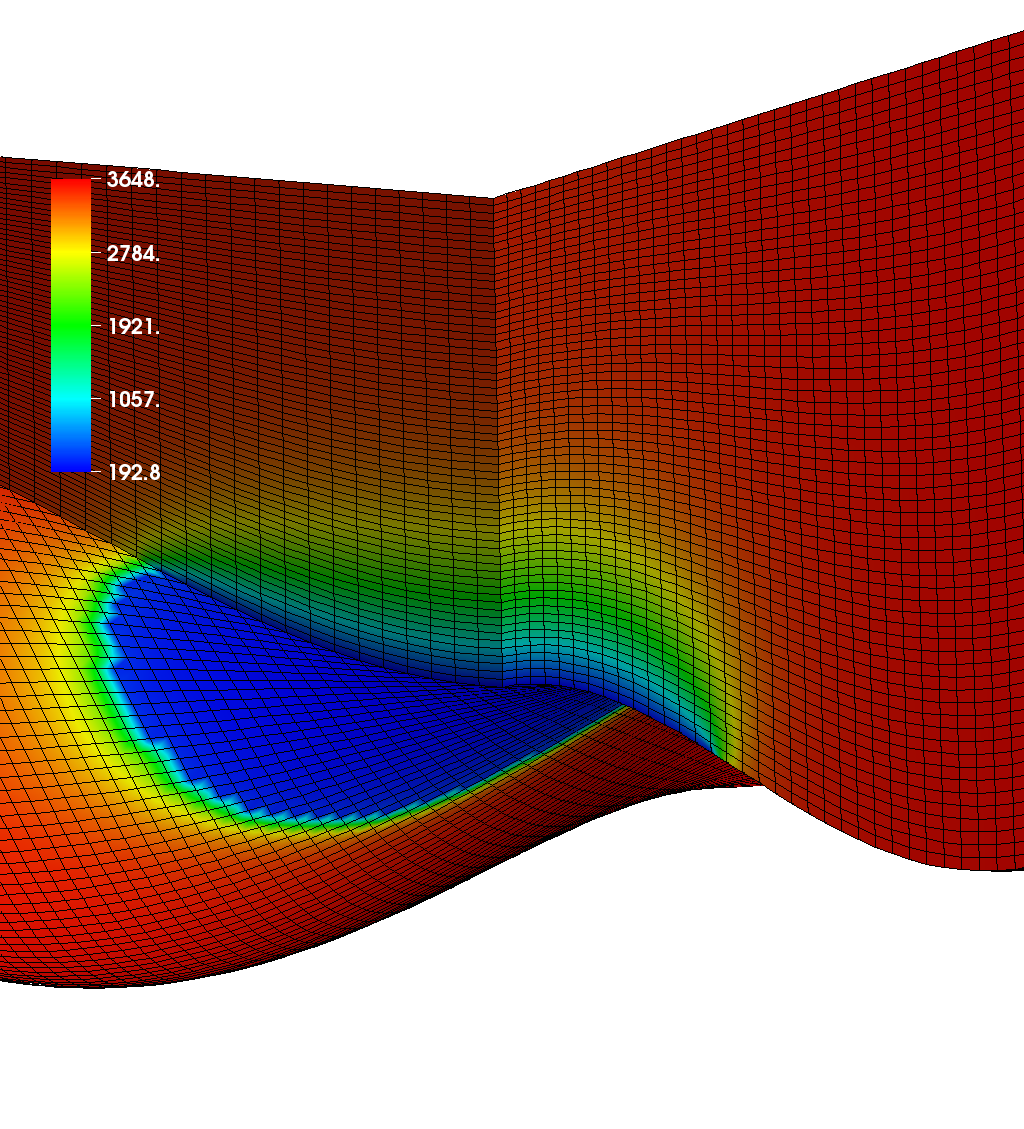
\includegraphics[width=1.2\textwidth]{figures/THI/x-5km-m8p5l5-clip}
}


\begin{frame}{Some Multigrid Options}
  \begin{itemize}
  \item \code{-dmmg\_grid\_sequencce}: [FALSE] \\
    Solve nonlinear problems on coarse grids to get initial guess
  \item \code{-pc\_mg\_galerkin}: [FALSE] \\
    Use Galerkin process to compute coarser operators
  \item \code{-pc\_mg\_type}: [FULL] \\
    (choose one of) MULTIPLICATIVE ADDITIVE FULL KASKADE
  \item \code{-mg\_coarse\_\{ksp,pc\}\_*} \\
    control the coarse-level solver
  \item \code{-mg\_levels\_\{ksp,pc\}\_*} \\
    control the smoothers on levels
  \item \code{-mg\_levels\_3\_\{ksp,pc\}\_*} \\
    control the smoother on specific level
  \item These also work with ML's algebraic multigrid.
  \end{itemize}
\end{frame}

\begin{frame}{What is this doing?}
\begin{itemize}
\item
\begin{alltt}\footnotesize
mpiexec -n 4 ./ex48
-M 16
-P 2
-da\_refine\_hierarchy\_x 1,8,8 \\
-da\_refine\_hierarchy\_y 2,1,1
-da\_refine\_hierarchy\_z 2,1,1 \\
-dmmg\_grid\_sequence 1
-dmmg\_view
-log\_summary \\
-ksp\_converged\_reason
-ksp\_gmres\_modifiedgramschmidt \\
-ksp\_monitor
-ksp\_rtol 1e-2 \\
-pc\_mg\_type multiplicative \\
-mg\_coarse\_pc\_type lu
-mg\_levels\_0\_pc\_type lu \\
-mg\_coarse\_pc\_factor\_mat\_solver\_package mumps \\
-mg\_levels\_0\_pc\_factor\_mat\_solver\_package mumps \\
-mg\_levels\_1\_sub\_pc\_type cholesky \\
-snes\_converged\_reason
-snes\_monitor
-snes\_stol 1e-12 \\
-thi\_L 80e3
-thi\_alpha 0.05
-thi\_friction\_m 0.3 \\
-thi\_hom x
-thi\_nlevels 4
\end{alltt}
\item What happens if you remove \code{-dmmg\_grid\_sequence}?
\item What about solving with block Jacobi, ASM, or algebraic multigrid?
\end{itemize}
\end{frame}

\subsection{Driven cavity}
\begin{frame}{SNES Example}
\framesubtitle{Driven Cavity}
\hbox{
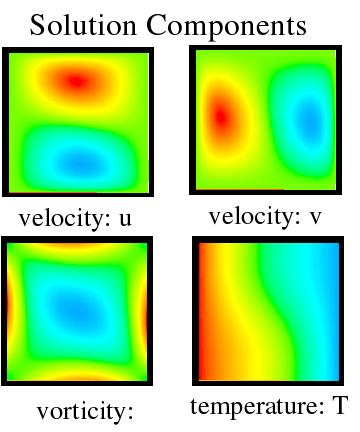
\includegraphics[width=.4\textwidth]{figures/SNES/DrivenCavitySolution}
\vbox{
\begin{itemize}
  \item Velocity-vorticity formulation
  \item Flow driven by lid and/or bouyancy
  \item Logically regular grid
  \begin{itemize}
    \item Parallelized with {\kb DMDA}
  \end{itemize}
  \item Finite difference discretization
  \item Authored by David Keyes
\end{itemize}
}
}
\code{src/snes/examples/tutorials/ex19.c}
\end{frame}

\begin{frame}[fragile]{SNES Example}
\framesubtitle{Driven Cavity Application Context}
\begin{minted}{c}
/* Collocated at each node */
typedef struct {
  PetscScalar u,v,omega,temp;
} Field;

typedef struct {
       /* physical parameters */
   PassiveReal lidvelocity,prandtl,grashof;
       /* color plots of the solution */
   PetscTruth  draw_contours;
} AppCtx;
\end{minted}
\end{frame}

\begin{frame}[fragile]{SNES Example}
\begin{minted}[fontsize=\footnotesize]{c}
DrivenCavityFunction(SNES snes, Vec X, Vec F, void *ptr) {
  AppCtx        *user = (AppCtx *) ptr;
  /* local starting and ending grid points */
  PetscInt       istart, iend, jstart, jend;
  PetscScalar    *f;             /* local vector data */
  PetscReal      grashof = user->grashof;  
  PetscReal      prandtl = user->prandtl;
  PetscErrorCode ierr;

  /* Code to communicate nonlocal ghost point data */
  VecGetArray(F, &f);

  /* Loop over local part and assemble into f[idxloc] */
  /* .... */

  VecRestoreArray(F, &f);
  return 0;
}
\end{minted}
\end{frame}

\begin{frame}[fragile]{SNES Example with local evaluation}
\begin{minted}[fontsize=\footnotesize]{c}
PetscErrorCode DrivenCavityFuncLocal(DMDALocalInfo *info,
                    Field **x,Field **f,void *ctx) {
  /* Handle boundaries ... */
  /* Compute over the interior points */
  for(j = info->ys; j < info->ys+info->ym; j++) {
    for(i = info->xs; i < info->xs+info->xm; i++) {
      /* convective coefficients for upwinding ... */
      /* U velocity */
      u          = x[j][i].u;
      uxx        = (2.0*u - x[j][i-1].u - x[j][i+1].u)*hydhx;
      uyy        = (2.0*u - x[j-1][i].u - x[j+1][i].u)*hxdhy;
      f[j][i].u  = uxx + uyy - .5*(x[j+1][i].omega-x[j-1][i].omega)*hx;
      /* V velocity, Omega ... */
      /* Temperature */
      u             = x[j][i].temp;
      uxx           = (2.0*u - x[j][i-1].temp - x[j][i+1].temp)*hydhx;
      uyy           = (2.0*u - x[j-1][i].temp - x[j+1][i].temp)*hxdhy;
      f[j][i].temp =  uxx + uyy + prandtl
        * (  (vxp*(u - x[j][i-1].temp) + vxm*(x[j][i+1].temp - u)) * hy
           + (vyp*(u - x[j-1][i].temp) + vym*(x[j+1][i].temp - u)) * hx);

}}}
\end{minted}

\begin{center}\small
\$PETSC\_DIR/src/snes/examples/tutorials/ex19.c
\end{center}
\end{frame}


\begin{frame}{Running the driven cavity}
  \begin{itemize}
  \item \code{./ex19 -lidvelocity 100 -grashof 1e2 -da\_grid\_x 16 -da\_grid\_y 16 -snes\_monitor -dmmg\_view -nlevels 3}
  \item \code{./ex19 -lidvelocity 100 -grashof 1e4 -da\_grid\_x 16 -da\_grid\_y 16 -snes\_monitor -dmmg\_view -nlevels 3}
  \item \code{./ex19 -lidvelocity 100 -grashof 1e5 -da\_grid\_x 16 -da\_grid\_y 16 -snes\_monitor -dmmg\_view -nlevels 3}
  \item<2-> Uh oh, we have convergence problems
  \item<2-> Run with \code{-snes\_monitor\_convergence}
  \item<2-> Does \code{-dmmg\_grid\_sequence} help? 
  \end{itemize}
\end{frame}

\begin{frame}{Why isn't SNES converging?}
  \begin{itemize}
  \item The Jacobian is wrong (maybe only in parallel)
    \oneitem{Check with \code{-snes\_type test} and \code{-snes\_mf\_operator -pc\_type lu}}
  \item The linear system is not solved accurately enough
    \begin{itemize}
    \item Check with \code{-pc\_type lu}
    \item Check \code{-ksp\_monitor\_true\_residual}, try right preconditioning
    \end{itemize}
  \item The Jacobian is singular with inconsistent right side
    \begin{itemize}
    \item Use \code{MatNullSpace} to inform the \code{KSP} of a known null space
    \item Use a different Krylov method or preconditioner
    \end{itemize}
  \item The nonlinearity is just really strong
    \begin{itemize}
    \item Run with \code{-info} or \code{-snes\_ls\_monitor} (petsc-dev) to see line search
    \item Try using trust region instead of line search \code{-snes\_type tr}
    \item Try grid sequencing if possible
    \item Use a continuation
    \end{itemize}
  \end{itemize}
\end{frame}

\begin{frame}{Globalizing the lid-driven cavity}
  \begin{block}{Pseudotransient continuation continuation ($\Psi tc$)}
    \begin{itemize}
    \item Do linearly implicit backward-Euler steps, driven by
      steady-state residual
    \item Clever way to adjust step sizes to retain quadratic
      convergence it terminal phase
    \end{itemize}
  \end{block}
  \begin{itemize}
  \item Implemented in \code{src/snes/examples/tutorials/ex27.c}
  \item \shell{make runex27}
  \item Make the method linearly implicit: \code{-snes\_max\_it 1}
    \oneitem{Compare required number of linear iterations}
  \item Try increasing \code{-lidvelocity}, \code{-grashof}, and problem size
  \item Coffey, Kelley, and Keyes, \emph{Pseudotransient continuation and differential algebraic equations}, SIAM J. Sci. Comp, 2003.
  \end{itemize}
\end{frame}


\section{Application Integration}
\begin{frame}{Application Integration}

\begin{itemize}
  \item Be willing to experiment with algorithms
  \begin{itemize}
    \item No optimality without interplay between physics and algorithmics
  \end{itemize}

  \item Adopt flexible, extensible programming
  \begin{itemize}
    \item Algorithms and data structures not hardwired
  \end{itemize}

  \item Be willing to play with the real code
  \begin{itemize}
    \item Toy models are rarely helpful
  \end{itemize}

  \item If possible, profile before integration
  \begin{itemize}
    \item Automatic in PETSc
  \end{itemize}
\end{itemize}

\end{frame}

\begin{frame}{Incorporating PETSc into existing codes}
  \begin{itemize}
  \item PETSc does not seize \code{main()}, does not control output
  \item Propogates errors from underlying packages, flexible error handling
  \item Nothing special about \code{MPI\_COMM\_WORLD}
  \item Can wrap existing data structures/algorithms
    \begin{itemize}
    \item \code{MatShell}, \code{PCShell}, full implementations
    \item \code{VecCreateMPIWithArray()}
    \item \code{MatCreateSeqAIJWithArrays()}
    \item Use an existing semi-implicit solver as a preconditioner
    \item Usually worthwhile to use native PETSc data structures \\
      unless you have a good reason not to
    \end{itemize}
  \item Uniform interfaces across languages
    \begin{itemize}
    \item C, C++, Fortran 77/90, Python, MATLAB
    \end{itemize}
  \item Do not have to use high level interfaces (\eg SNES, TS, DM)
    \begin{itemize}
    \item but PETSc can offer more if you do, like MFFD and SNES Test
    \end{itemize}
  \end{itemize}
\end{frame}

\begin{frame}{Integration Stages}

\begin{itemize}
  % I like the simile of VC as a will. It cheap, easy, someone will help you,
  % and if you die you are an idiot for not using one
  \item \red{Version Control}
  \begin{itemize}
    \item It is impossible to overemphasize
  \end{itemize}

  \item Initialization
  \begin{itemize}
    \item Linking to PETSc
  \end{itemize}

  \item Profiling
  \begin{itemize}
    \item Profile \red{before} changing
    \item Also incorporate command line processing
  \end{itemize}

  \item Linear Algebra
  \begin{itemize}
    \item First PETSc data structures
  \end{itemize}

  \item Solvers
  \begin{itemize}
    \item Very easy after linear algebra is integrated
  \end{itemize}
\end{itemize}

\end{frame}

\begin{frame}{Initialization}

\begin{itemize}
  \item Call {\kb PetscInitialize()}
  \begin{itemize}
    \item Setup static data and services
    \item Setup MPI if it is not already
    \item Can set \code{PETSC\_COMM\_WORLD} to use your communicator \\
      (can always use subcommunicators for each object)
  \end{itemize}

  \item Call {\kb PetscFinalize()}
  \begin{itemize}
    \item Calculates logging summary
    \item Can check for leaks/unused options
    \item Shutdown and release resources
  \end{itemize}

  \item Can only initialize PETSc once
\end{itemize}

\end{frame}

\begin{frame}{Matrix Memory Preallocation}
\begin{itemize}
  \item PETSc sparse matrices are dynamic data structures
  \begin{itemize}
    \item can add additional nonzeros freely
  \end{itemize}

  \item Dynamically adding many nonzeros 
  \begin{itemize}
    \item requires additional memory allocations
    \item requires copies
    \item can kill performance
  \end{itemize}

  \item Memory preallocation provides
  \begin{itemize}
    \item the freedom of dynamic data structures
    \item good performance
  \end{itemize}

  \item Easiest solution is to replicate the assembly code
  \begin{itemize}
    \item Remove computation, but preserve the indexing code
    \item Store set of columns for each row
  \end{itemize}

  \item Call preallocation routines for all datatypes
  \begin{itemize}
    \item {\kb MatSeqAIJSetPreallocation()}
    \item {\kb MatMPIBAIJSetPreallocation()}
    \item Only the relevant data will be used
  \end{itemize}
\end{itemize}
\end{frame}

\begin{frame}{Sequential Sparse Matrices}
{\kb MatSeqAIJSetPreallocation(Mat A, int nz, int nnz[])}
\hbox{\qquad
\vbox{
\begin{itemize}
  \item[nz:] expected number of nonzeros in any row
  \item[nnz(i):] expected number of nonzeros in row i
\end{itemize}
}
}

\begin{center}
%\includegraphics[width=2in]{figures/Mat/serialSparseMatrix_bcsstk32}
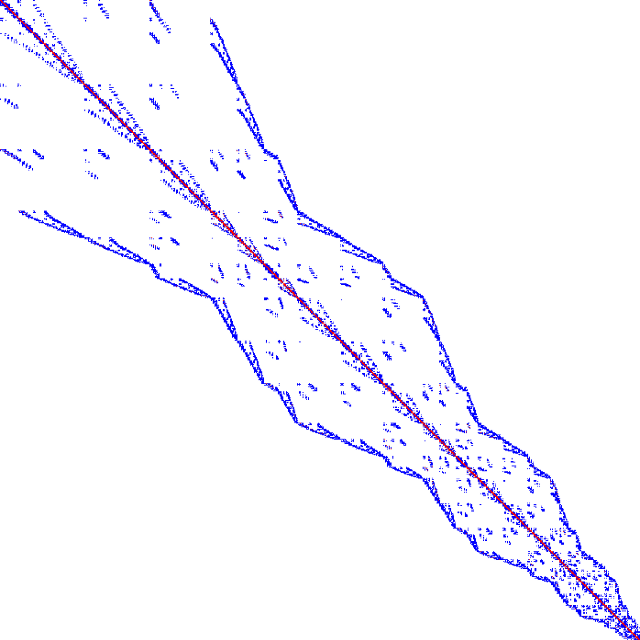
\includegraphics[width=.5\textwidth]{figures/EllipRCMSquare}
\end{center}
\end{frame}

\begin{frame}{Parallel Sparse Matrix}
\begin{itemize}
  \item Each process locally owns a submatrix of contiguous global rows
  \item Each submatrix consists of diagonal and off-diagonal parts
\end{itemize}

\begin{center}
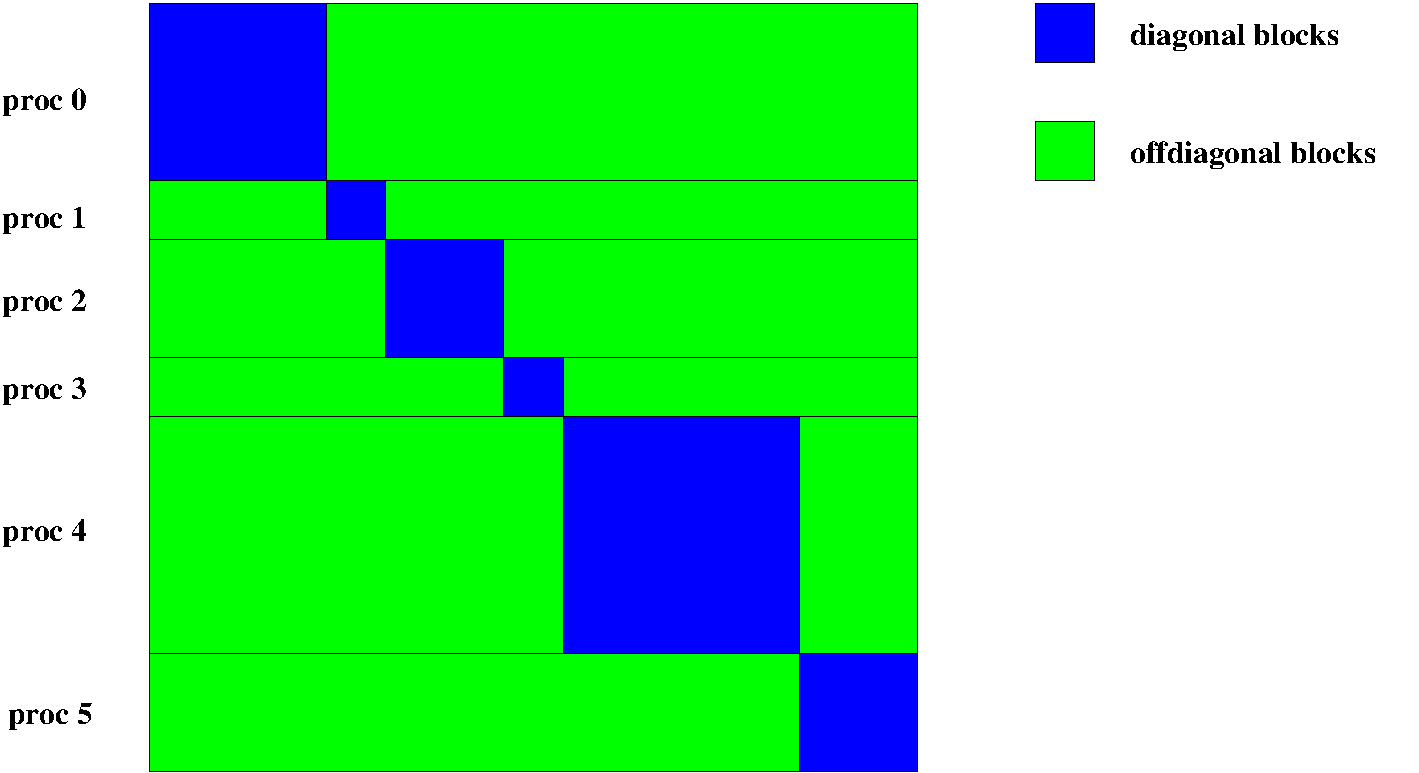
\includegraphics[width=3.5in]{figures/Mat/parallelSparseMatrix}
\end{center}

\begin{itemize}
  \item {\kb MatGetOwnershipRange(Mat A,int *start,int *end)}
  \begin{itemize}
    \item[{\kb start}:] first locally owned row of global matrix
    \item[{\kb end-1}:] last locally owned row of global matrix
  \end{itemize}
\end{itemize}
\end{frame}

\begin{frame}{Parallel Sparse Matrices}
\hbox{
\quad
\vbox{
{\kb MatMPIAIJSetPreallocation(Mat A, int dnz, int dnnz[], \\
  \qquad \qquad int onz, int onnz[])}
\begin{itemize}
  \item[dnz:] expected number of nonzeros in any row in the diagonal block
  \item[dnnz(i):] expected number of nonzeros in row i in the diagonal block
  \item[onz:] expected number of nonzeros in any row in the offdiagonal portion
  \item[onnz(i):] expected number of nonzeros in row i in the offdiagonal portion
\end{itemize}
}
}
\end{frame}

\begin{frame}{Verifying Preallocation}
\begin{itemize}
  \item Use runtime options \\
    {\kb -mat\_new\_nonzero\_location\_err} \\
    {\kb -mat\_new\_nonzero\_allocation\_err}
  \item Use runtime option {\kb -info}
  \item Output: \\
{\kb
  $[$proc \#$]$ Matrix size: \%d X \%d; storage space: \%d unneeded, \%d used \\
  $[$proc \#$]$ Number of mallocs during MatSetValues( )  is \%d
}
\end{itemize}

\bigskip

\begin{center}
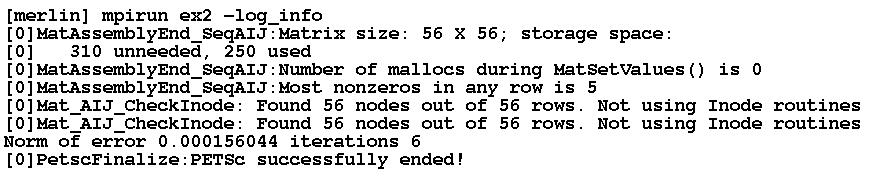
\includegraphics[width=5in]{figures/PETSc/logInfoOutput}
\end{center}
\end{frame}

\begin{frame}{Block and symmetric formats}
  \begin{itemize}
  \item BAIJ
    \begin{itemize}
    \item Like AIJ, but uses static block size
    \item Preallocation is like AIJ, but just one index per block
    \end{itemize}
  \item SBAIJ
    \begin{itemize}
    \item Only stores upper triangular part
    \item Preallocation needs number of nonzeros in upper triangular \\
      parts of on- and off-diagonal blocks
    \end{itemize}
  \item \code{MatSetValuesBlocked()}
    \begin{itemize}
    \item Better performance with blocked formats
    \item Also works with scalar formats, if \code{MatSetBlockSize()} was called
    \item Variants \code{MatSetValuesBlockedLocal()}, \code{MatSetValuesBlockedStencil()}
    \item Change matrix format at runtime, don't need to touch assembly code
    \end{itemize}
  \end{itemize}
\end{frame}

\begin{frame}{Linear Solvers}{Krylov Methods}

\begin{itemize}
  \item Using PETSc linear algebra, just add:
  \begin{itemize}
    \item {\kb KSPSetOperators(KSP ksp, Mat A, Mat M, MatStructure flag)}
    \item {\kb KSPSolve(KSP ksp, Vec b, Vec x)}
  \end{itemize}

  \item Can access subobjects
  \begin{itemize}
    \item {\kb KSPGetPC(KSP ksp, PC *pc)}
  \end{itemize}

  \item Preconditioners must obey PETSc interface
  \begin{itemize}
    \item Basically just the KSP interface
  \end{itemize}

  \item Can change solver dynamically from the command line, {\kb -ksp\_type}
\end{itemize}

\end{frame}

\begin{frame}{Nonlinear Solvers}{Newton and Picard Methods}

\begin{itemize}
  \item Using PETSc linear algebra, just add:
  \begin{itemize}
    \item {\kb SNESSetFunction(SNES snes, Vec r, residualFunc, void *ctx)}
    \item {\kb SNESSetJacobian(SNES snes, Mat A, Mat M, jacFunc, void *ctx)}
    \item {\kb SNESSolve(SNES snes, Vec b, Vec x)}
  \end{itemize}

  \item Can access subobjects
  \begin{itemize}
    \item {\kb SNESGetKSP(SNES snes, KSP *ksp)}
  \end{itemize}

  \item Can customize subobjects from the cmd line
  \begin{itemize}
    \item Set the subdomain preconditioner to ILU with {\kb -sub\_pc\_type ilu} 
  \end{itemize}
\end{itemize}

\end{frame}


\section{Performance and Scalability}
%\input{WhyWeNeedAPerformanceModel.tex}
\begin{frame}{Bottlenecks of (Jacobian-free) Newton-Krylov}
  \begin{columns}
    \begin{column}{0.4\textwidth}
      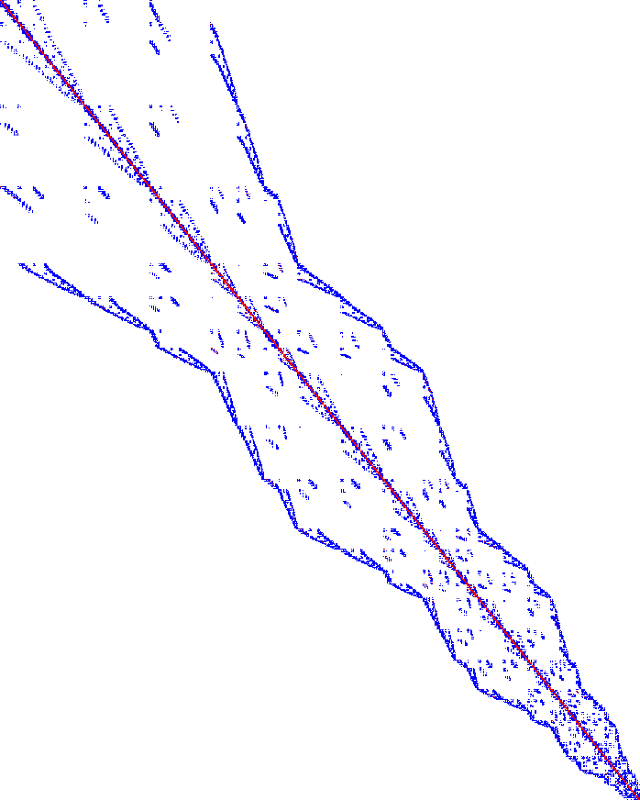
\includegraphics[width=1.15\textwidth]{figures/Dohp/EllipRCM}
    \end{column}
    \begin{column}{0.6\textwidth}
      \begin{itemize}
      \item Matrix assembly
        \begin{itemize}
        \item integration/fluxes: FPU
        \item insertion: memory/branching
        \end{itemize}
      \item Preconditioner setup
        \begin{itemize}
        \item coarse level operators
        \item overlapping subdomains
        \item (incomplete) factorization
        \end{itemize}
      \item Preconditioner application
        \begin{itemize}
        \item triangular solves/relaxation: memory
        \item coarse levels: network latency
        \end{itemize}
      \item Matrix multiplication
        \begin{itemize}
        \item Sparse storage: memory
        \item Matrix-free: FPU
        \end{itemize}
      \item Globalization
      \end{itemize}
    \end{column}
  \end{columns}
\end{frame}

\subsection{Memory hierarchy}
\begin{frame} %{CPU Architecture}
  \begin{columns}
    \begin{column}{0.5\textwidth}
      {\centering Intel Clowertown \\
      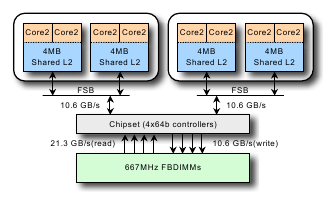
\includegraphics[width=\textwidth]{figures/hardware/IntelClovertown} }
    \begin{itemize}
    \item 75 Gflop/s
    \item 21 GB/s bandwidth
    \item thread + instruction level parallelism
    \item vector instructions (SSE)
    \end{itemize}
    \end{column}
    \begin{column}{0.5\textwidth}
      {\centering       AMD Opteron \\
      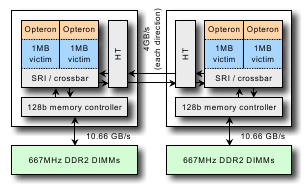
\includegraphics[width=\textwidth]{figures/hardware/AMDOpteron} }
    \begin{itemize}
    \item 17 Gflop/s
    \item 21 GB/s bandwidth
    \item thread + instruction level parallelism
    \item vector instructions (SSE)
    \end{itemize}
    \end{column}
  \end{columns}
\end{frame}

\begin{frame}{Hardware capabilities}
  \begin{columns}
    \begin{column}{0.5\textwidth}
      \begin{block}{Floating point unit}
        Recent Intel: each core can issue
        \begin{itemize}
        \item 1 packed add (latency 3)
        \item 1 packed mult (latency 5)
        \item One can include an aligned read
        \item Out of Order execution
        \item Peak: 10 Gflop/s (\texttt{double})
        \end{itemize}
      \end{block}
    \end{column}
    \begin{column}{0.5\textwidth}
      \begin{block}{Memory}
        \begin{itemize}
        \item $\sim 250$ cycle latency
        \item 5.3 GB/s bandwidth
        \item 1 \texttt{double} load / 3.7 cycles
        \item Pay by the cache line (32/64 B)
        \item L2 cache: $\sim 10$ cycle latency
        \end{itemize}
      \end{block}
    \end{column}
  \end{columns}
  \begin{block}{}%<2>{\alert{\Large It's \textbf{all} about the memory hierarchy}}
    \centering
    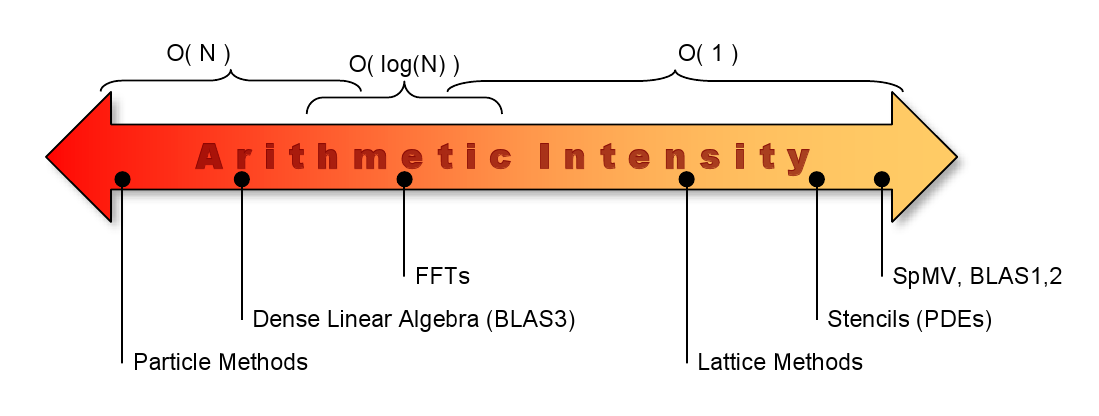
\includegraphics[width=0.85\textwidth]{figures/OlikerArithmeticIntensity} \\
    \vspace{-1em}
    {\tiny (Oliker et al. 2008)}
  \end{block}
\end{frame}

\frame{
  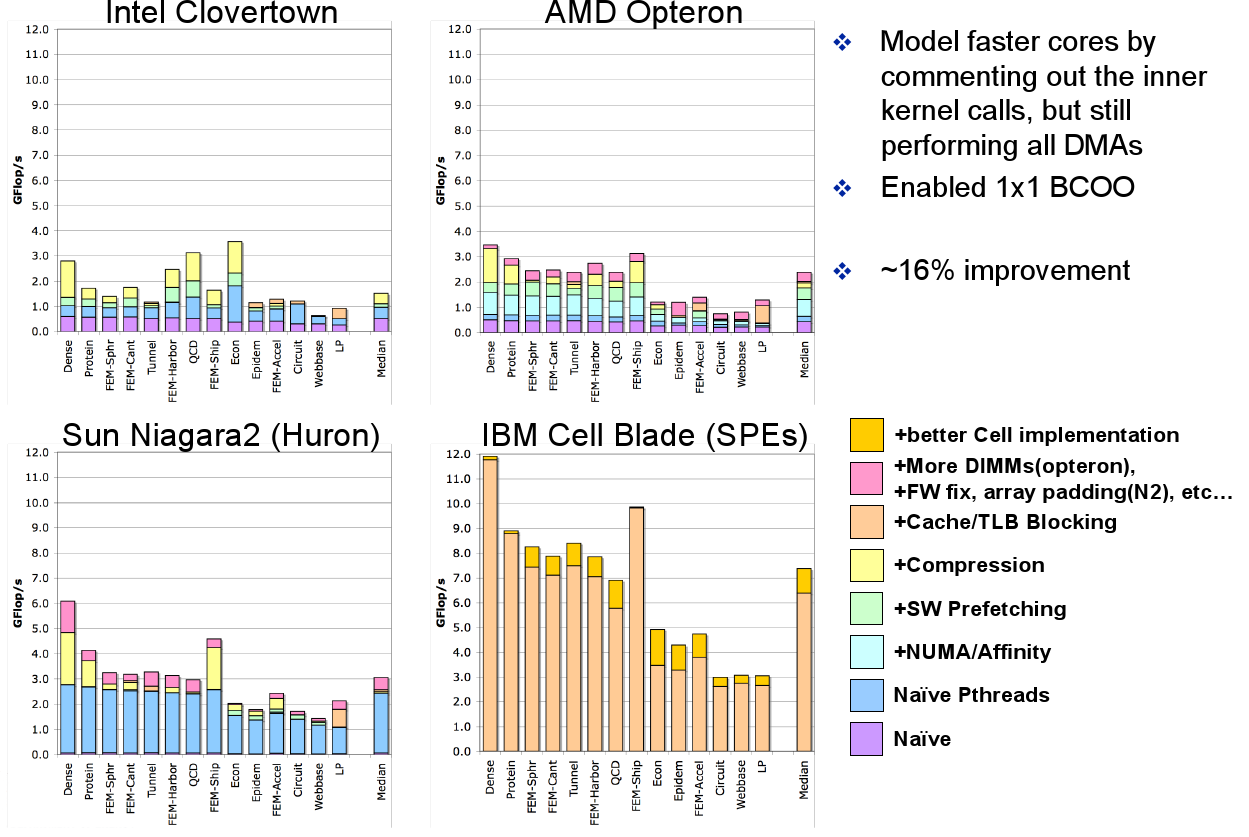
\includegraphics[width=\textwidth]{figures/OlikerSpMv} \\
  {\tiny (Oliker et al. \emph{Multi-core Optimization of Sparse Matrix Vector Multiplication}, 2008)}
}

\begin{frame}[fragile]{Sparse Mat-Vec performance model}
  \begin{block}{Compressed Sparse Row format (AIJ)}
    For $m \times n$ matrix with $N$ nonzeros
    \begin{itemize}
    \item[ai] row starts, length $m+1$
    \item[aj] column indices, length $N$, range $[0,n-1)$
    \item[aa] nonzero entries, length $N$, scalar values
    \end{itemize}
  \end{block}
\begin{columns}
\begin{column}{0.3\textwidth}
\[y \gets y + A x\]
\end{column}
\begin{column}{0.7\textwidth}
\begin{lstlisting}
  for (i=0; i<m; i++)
    for (j=ai[i]; j<ai[i+1]; j++)
      y[i] += aa[j] * x[aj[j]];
    \end{lstlisting}
  \end{column}
\end{columns}
  \begin{itemize}
  \item One add and one multiply per inner loop
  \item Scalar \code{aa[j]} and integer \code{aj[j]} only used once
  \item Must load \code{aj[j]} to read from \code{x}, may not reuse cache well
  \end{itemize}
\end{frame}

\begin{frame}[shrink=1]{Memory Bandwidth}
\begin{itemize}
\item Stream Triad benchmark (GB/s): $\bm w \gets \alpha \bm x + \bm y$
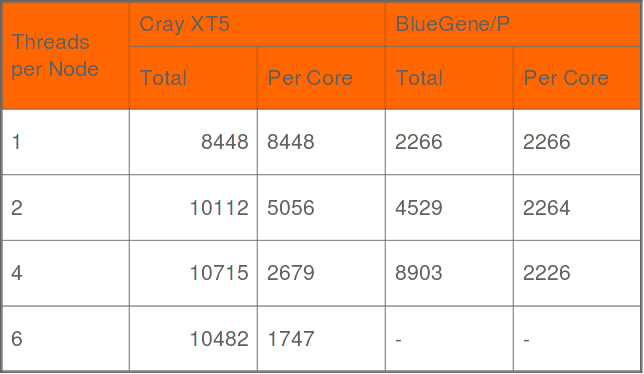
\includegraphics[width=0.8\textwidth]{figures/StreamTriadXT5VsBGP} \\
\item Sparse matrix-vector product: 6 bytes per flop
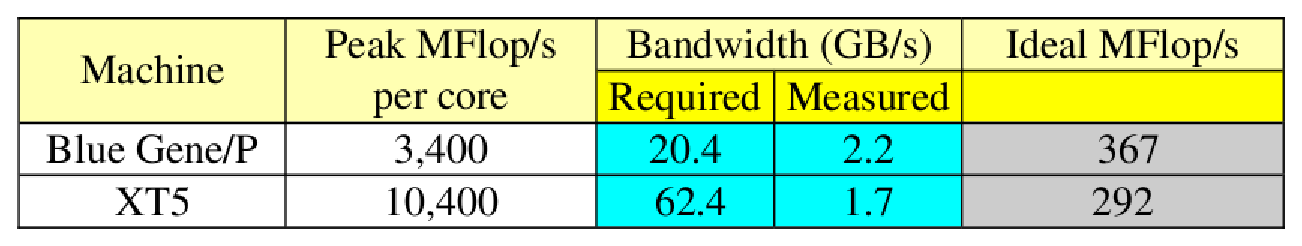
\includegraphics[width=0.8\textwidth]{figures/SparseMatVec} \\
%{\footnotesize (from Dinesh Kaushik)}
\end{itemize}
\end{frame}



\begin{frame}{Optimizing Sparse Mat-Vec}
  \begin{itemize}
  \item Order unknows so that vector reuses cache (Reverse Cuthill-McKee)
    \begin{itemize}
    \item Optimal: $\frac{(2 \text{ flops})(\text{bandwidth})}{\texttt{sizeof(Scalar)} + \texttt{sizeof(Int)}}$
    \item Usually improves strength of ILU and SOR
    \end{itemize}
  \item Coalesce indices for adjacent rows with same nonzero pattern (Inodes)
    \begin{itemize}
    \item Optimal: $\frac{(2 \text{ flops})(\text{bandwidth})}{\texttt{sizeof(Scalar)} + \texttt{sizeof(Int)}/i}$
    \item Can do block SOR (much stronger than scalar SOR)
    \item Default in PETSc, turn off with \code{-mat\_no\_inode}
    \item Requires ordering unknowns so that fields are interlaced, this
      is (much) better for memory use anyway
    \end{itemize}
  \item Use explicit blocking, hold one index per block (BAIJ format)
    \begin{itemize}
    \item Optimal: $\frac{(2 \text{ flops})(\text{bandwidth})}{\texttt{sizeof(Scalar)} + \texttt{sizeof(Int)}/b^2}$
    \item Block SOR and factorization
    \item Symbolic factorization works with blocks (much cheaper)
    \item Very regular memory access, unrolled dense kernels
    \item Faster insertion: \code{MatSetValuesBlocked()}
    \end{itemize}
  \end{itemize}
\end{frame}

\begin{frame}{Optimizing unassembled Mat-Vec}
  \begin{itemize}
  \item High order spatial discretizations do more work per node
    \begin{itemize}
    \item Dense tensor product kernel (like small BLAS3)
    \item Cubic ($Q_3$) elements in 3D can achieve $>60\%$ of peak FPU \\
      (compare to $< 6\%$ for assembled operators on multicore)
    \item Can store Jacobian information at quadrature points \\
      (usually pays off for $Q_2$ and higher in 3D)
    \item Spectral methods
    \item Often still need an assembled operator for preconditioning
    \end{itemize}
  \item Boundary element methods
    \begin{itemize}
    \item Dense kernels
    \item Fast Multipole Method (FMM)
    \end{itemize}
  \end{itemize}
\end{frame}

%\subsection{Matrix formats}
%\input{MatrixPreallocation}
%\frame{}
%\subsubsection{Preallocation}
%\frame{}
\subsection{Profiling}
\begin{frame}{Profiling}

\begin{itemize}
  \item Use {\kb -log\_summary} for a performance profile
  \begin{itemize}
    \item Event timing
    \item Event flops
    \item Memory usage
    \item MPI messages
  \end{itemize}

  \item Call {\kb PetscLogStagePush()} and {\kb PetscLogStagePop()}
  \begin{itemize}
    \item User can add new stages
  \end{itemize}

  \item Call {\kb PetscLogEventBegin()} and {\kb PetscLogEventEnd()}
  \begin{itemize}
    \item User can add new events
  \end{itemize}

  \item Call {\kb PetscLogFlops()} to include your flops
\end{itemize}

\end{frame}

\begin{frame}[fragile]{Reading \code{-log\_summary}}
\begin{itemize}
\item
{\scriptsize
\begin{verbatim}
                         Max       Max/Min        Avg      Total 
Time (sec):           1.548e+02      1.00122   1.547e+02
Objects:              1.028e+03      1.00000   1.028e+03
Flops:                1.519e+10      1.01953   1.505e+10  1.204e+11
Flops/sec:            9.814e+07      1.01829   9.727e+07  7.782e+08
MPI Messages:         8.854e+03      1.00556   8.819e+03  7.055e+04
MPI Message Lengths:  1.936e+08      1.00950   2.185e+04  1.541e+09
MPI Reductions:       2.799e+03      1.00000
\end{verbatim}}
\item Also a summary per stage
\item Memory usage per stage (based on when it was allocated)
\item Time, messages, reductions, balance, flops per event per stage
\item Always send \code{-log\_summary} when asking \\
  performance questions on mailing list
\end{itemize}
\end{frame}

\begin{frame}[fragile]{Reading \code{-log\_summary}}
\begin{Verbatim}[formatcom=\tiny]
Event                Count      Time (sec)     Flops                             --- Global ---  --- Stage ---   Total
                   Max Ratio  Max     Ratio   Max  Ratio  Mess   Avg len Reduct  %T %F %M %L %R  %T %F %M %L %R Mflop/s
------------------------------------------------------------------------------------------------------------------------
--- Event Stage 1: Full solve
VecDot                43 1.0 4.8879e-02 8.3 1.77e+06 1.0 0.0e+00 0.0e+00 4.3e+01  0  0  0  0  0   0  0  0  0  1 73954
VecMDot             1747 1.0 1.3021e+00 4.6 8.16e+07 1.0 0.0e+00 0.0e+00 1.7e+03  0  1  0  0 14   1  1  0  0 27 128346
VecNorm             3972 1.0 1.5460e+00 2.5 8.48e+07 1.0 0.0e+00 0.0e+00 4.0e+03  0  1  0  0 31   1  1  0  0 61 112366
VecScale            3261 1.0 1.6703e-01 1.0 3.38e+07 1.0 0.0e+00 0.0e+00 0.0e+00  0  0  0  0  0   0  0  0  0  0 414021
VecScatterBegin     4503 1.0 4.0440e-01 1.0 0.00e+00 0.0 6.1e+07 2.0e+03 0.0e+00  0  0 50 26  0   0  0 96 53  0     0
VecScatterEnd       4503 1.0 2.8207e+00 6.4 0.00e+00 0.0 0.0e+00 0.0e+00 0.0e+00  0  0  0  0  0   0  0  0  0  0     0
MatMult             3001 1.0 3.2634e+01 1.1 3.68e+09 1.1 4.9e+07 2.3e+03 0.0e+00 11 22 40 24  0  22 44 78 49  0 220314
MatMultAdd           604 1.0 6.0195e-01 1.0 5.66e+07 1.0 3.7e+06 1.3e+02 0.0e+00  0  0  3  0  0   0  1  6  0  0 192658
MatMultTranspose     676 1.0 1.3220e+00 1.6 6.50e+07 1.0 4.2e+06 1.4e+02 0.0e+00  0  0  3  0  0   1  1  7  0  0 100638
MatSolve            3020 1.0 2.5957e+01 1.0 3.25e+09 1.0 0.0e+00 0.0e+00 0.0e+00  9 21  0  0  0  18 41  0  0  0 256792
MatCholFctrSym         3 1.0 2.8324e-04 1.0 0.00e+00 0.0 0.0e+00 0.0e+00 0.0e+00  0  0  0  0  0   0  0  0  0  0     0
MatCholFctrNum        69 1.0 5.7241e+00 1.0 6.75e+08 1.0 0.0e+00 0.0e+00 0.0e+00  2  4  0  0  0   4  9  0  0  0 241671
MatAssemblyBegin     119 1.0 2.8250e+00 1.5 0.00e+00 0.0 2.1e+06 5.4e+04 3.1e+02  1  0  2 24  2   2  0  3 47  5     0
MatAssemblyEnd       119 1.0 1.9689e+00 1.4 0.00e+00 0.0 2.8e+05 1.3e+03 6.8e+01  1  0  0  0  1   1  0  0  0  1     0
SNESSolve              4 1.0 1.4302e+02 1.0 8.11e+09 1.0 6.3e+07 3.8e+03 6.3e+03 51 50 52 50 50  99100 99100 97 113626
SNESLineSearch        43 1.0 1.5116e+01 1.0 1.05e+08 1.1 2.4e+06 3.6e+03 1.8e+02  5  1  2  2  1  10  1  4  4  3 13592
SNESFunctionEval      55 1.0 1.4930e+01 1.0 0.00e+00 0.0 1.8e+06 3.3e+03 8.0e+00  5  0  1  1  0  10  0  3  3  0     0
SNESJacobianEval      43 1.0 3.7077e+01 1.0 7.77e+06 1.0 4.3e+06 2.6e+04 3.0e+02 13  0  4 24  2  26  0  7 48  5   429
KSPGMRESOrthog      1747 1.0 1.5737e+00 2.9 1.63e+08 1.0 0.0e+00 0.0e+00 1.7e+03  1  1  0  0 14   1  2  0  0 27 212399
KSPSetup             224 1.0 2.1040e-02 1.0 0.00e+00 0.0 0.0e+00 0.0e+00 3.0e+01  0  0  0  0  0   0  0  0  0  0     0
KSPSolve              43 1.0 8.9988e+01 1.0 7.99e+09 1.0 5.6e+07 2.0e+03 5.8e+03 32 49 46 24 46  62 99 88 48 88 178078
PCSetUp              112 1.0 1.7354e+01 1.0 6.75e+08 1.0 0.0e+00 0.0e+00 8.7e+01  6  4  0  0  1  12  9  0  0  1 79715
PCSetUpOnBlocks     1208 1.0 5.8182e+00 1.0 6.75e+08 1.0 0.0e+00 0.0e+00 8.7e+01  2  4  0  0  1   4  9  0  0  1 237761
PCApply              276 1.0 7.1497e+01 1.0 7.14e+09 1.0 5.2e+07 1.8e+03 5.1e+03 25 44 42 20 41  49 88 81 39 79 200691
\end{Verbatim}
\end{frame}

\begin{frame}{Communication Costs}
  \begin{itemize}
  \item Reductions: usually part of Krylov method, latency limited
    \begin{itemize}
    \item \code{VecDot}
    \item \code{VecMDot}
    \item \code{VecNorm}
    \item \code{MatAssemblyBegin}
    \item Change algorithm (e.g. IBCGS)
    \end{itemize}
  \item Point-to-point (nearest neighbor), latency or bandwidth
    \begin{itemize}
    \item \code{VecScatter}
    \item \code{MatMult}
    \item \code{PCApply}
    \item \code{MatAssembly}
    \item \code{SNESFunctionEval}
    \item \code{SNESJacobianEval}
    \item Compute subdomain boundary fluxes redundantly
    \item Ghost exchange for all fields at once
    \item Better partition
    \end{itemize}
  \end{itemize}
\end{frame}

\begin{frame}{Scalability definitions}
  \begin{columns}
    \begin{column}{0.5\textwidth}
      {\large Strong scalability}
      \begin{itemize}
      \item Fixed problem size
      \item execution time $T$ inversely proportional to number of processors $p$
      \end{itemize}
    \end{column}
    \begin{column}{0.5\textwidth}
      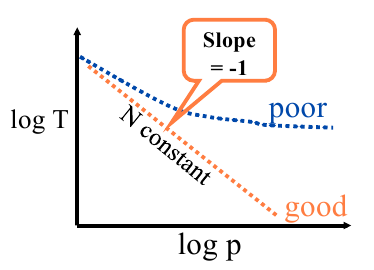
\includegraphics[width=\textwidth]{figures/KeyesStrongScaling.png}
    \end{column}
  \end{columns}
  \begin{columns}
    \begin{column}{0.5\textwidth}
      {\large Weak scalability}
      \begin{itemize}
      \item Fixed problem size per processor
      \item execution time constant as problem size increases
      \end{itemize}
    \end{column}
    \begin{column}{0.5\textwidth}
      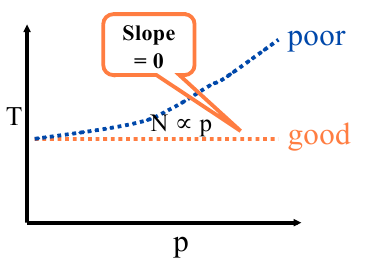
\includegraphics[width=\textwidth]{figures/KeyesWeakScaling.png}
    \end{column}
  \end{columns}
\end{frame}

\begin{frame}{Multigrid advice}
  \begin{itemize}
  \item Rapid coarsening is essential for weak scalability
    \begin{itemize}
    \item Push the algorithm towards ``multilevel domain decomposition''
    \end{itemize}
  \item Energy minimizing interpolants
    \begin{itemize}
    \item Similar to exotic Schwarz methods, see Dohrmann and Widlund 2008, 2009
    \item Closely related to FETI-DP/BDDC coarse spaces
    \end{itemize}
  \item Interpolation operators must be compatible with physics (e.g. inf-sup conditions)
  \item Ordering of unknowns can make incomplete factorization behave \\
    similar to line smoothers
  \item Nonlinear multigrid (FAS) is worth trying if pointwise or block \\
    residuals are cheap, or globalization is especially challenging
  \item Monotone multigrid (Kornhuber) for variational inequalities
  \item Boundary conditions in subdomain problems (``optimized Schwarz'')
  \end{itemize}
\end{frame}


\section{Hard problems}
\begin{frame}{Splitting for Multiphysics}
  \begin{equation*}
    \begin{bmatrix}
      A & B \\ C & D
    \end{bmatrix}
    \begin{bmatrix}
      x \\ y
    \end{bmatrix}
    =
    \begin{bmatrix}
      f \\ g
    \end{bmatrix}
  \end{equation*}
  \begin{itemize}\item Relaxation:
    \code{-pc\_fieldsplit\_type [additive,multiplicative,symmetric\_multiplicative]}
    \begin{equation*}
      \begin{bmatrix}
        A & \\  & D
      \end{bmatrix}^{-1} \qquad 
      \begin{bmatrix}
        A & \\ C & D
      \end{bmatrix}^{-1} \qquad
      \begin{bmatrix}
        A & \\  & \bm 1
      \end{bmatrix}^{-1}
      \left(
        \bm 1 -
        \begin{bmatrix}
          A & B \\ & \bm 1
        \end{bmatrix}
        \begin{bmatrix}
          A & \\ C & D
        \end{bmatrix}^{-1}
      \right)
    \end{equation*}
    \begin{itemize}
    \item Gauss-Seidel inspired, works when fields are loosely coupled
    \end{itemize}
  \item Factorization: \code{-pc\_fieldsplit\_type schur}
    \begin{align*}
      \begin{bmatrix}
        A & B \\ & S
      \end{bmatrix}^{-1}
      \begin{bmatrix}
        1 & \\ CA^{-1} & 1
      \end{bmatrix}^{-1}, \qquad
      S = D - C A^{-1} B
    \end{align*}
    \begin{itemize}
    \item robust (exact factorization), can often drop lower block
    \item how to precondition $S$ which is usually dense?
      \begin{itemize}
      \item interpret as differential operators, use approximate commutators
      \end{itemize}
    \end{itemize}
  \end{itemize}
\end{frame}

\begin{frame}{Coupled approach to multiphysics}
  \begin{itemize}
  \item Smooth all components together
    \begin{itemize}
    \item Block SOR is the most popular
    \item Block ILU sometimes more robust (\eg transport/anisotropy)
    \item Vanka field-split smoothers or for saddle-point problems
    \item Distributive relaxation
    \end{itemize}
  \item Scaling between fields is critical
  \item Indefiniteness
    \begin{itemize}
    \item Make smoothers and interpolants respect inf-sup condition
    \item Difficult to handle anisotropy
    \item Exotic interpolants for Helmholtz
    \end{itemize}
  \item Transport
    \begin{itemize}
    \item Define smoother in terms of first-order upwind discretization ($h$-ellipticity)
    \item Evaluate residuals using high-order discretization
    \item Use Schur field-split: ``parabolize'' at top level or for smoother on levels
    \end{itemize}
  \item Multigrid inside field-split or field-split inside multigrid
  \item Open research area, hard to write modular software
  \end{itemize}
\end{frame}

\begin{frame}{Anisotropy and Heterogeneity}
  \begin{itemize}
  \item Anisotropy
    \begin{itemize}
    \item Semi-coarsening
    \item Line smoothers
    \item Order unknowns so that incomplete factorization ``includes'' a
      line smoother
    \end{itemize}
  \item Heterogeneity
    \begin{itemize}
    \item Make coarse grids align
    \item Strong smoothers
    \item Energy-minimizing interpolants
    \end{itemize}
  \end{itemize}
\end{frame}

\begin{frame}[shrink=10]{``Physics-based'' preconditioners (semi-implicit method)}
  \begin{block}{Shallow water with stiff gravity wave}
    $h$ is hydrostatic pressure, $u$ is velocity, $\sqrt{gh}$ is fast wave speed
    \begin{gather*}
      h_t - (uh)_x = 0 \\
      (uh)_t + (u^2h + \half gh^2)_x = 0
    \end{gather*}
  \end{block}
  \vspace{-3em}
  \begin{block}{Semi-implicit method}
    Suppress spatial discretization, discretize in time, implicitly for the terms contributing to the gravity wave
    \begin{gather*}
      \frac{h^{n+1} - h^n}{\Delta t} + (uh)_x^{n+1} = 0 \\
      \frac{(uh)^{n+1} - (uh)^{n}}{\Delta t} + (u^2h)_x^{n} + g(h^n h^{n+1})_x = 0
    \end{gather*}

    Rearrange, eliminating $(uh)^{n+1}$
    \[ \frac{h^{n+1} - h^n}{\Delta t} - \Delta t(gh^n h_x^{n+1})_x = -S_x^n \]
  \end{block}
\end{frame}

\begin{frame}[shrink=1]{Delta form}
  \begin{itemize}
  \item Preconditioner should work like the Newton step: $-F(x) \mapsto \delta x$
  \item Recast semi-implicit method in delta form
    \[ \frac{\delta h}{\Delta t} + (\delta uh)_x = -F_0, \quad \frac{\delta uh}{\Delta t} + g h^n (\delta h)_x = -F_1,
    \quad \widehat{J} =
    \begin{pmatrix}
      \frac{1}{\Delta t} & \div \\
      g h^n \nabla & \frac{1}{\Delta t}
    \end{pmatrix}
    \]
  \item Eliminate $\delta uh$
    \[ \frac{\delta h}{\Delta t} - \Delta t(gh^n (\delta h)_x)_x = -F_0 + (\Delta t F_1)_x,
    \quad S \sim \frac{1}{\Delta t} - g \Delta t \div h^n \nabla
    \]
  \item Solve for $\delta h$, then evaluate
    \[ \delta uh = - \Delta t \big[ gh^n (\delta h)_x - F_1 \big] \]
  \item Fully implicit solver
    \begin{itemize}
    \item Is nonlinearly consistent (no splitting error), can be high-order in time
    \item Uses existing code when a semi-implicit method has been implemented
    \item Allows efficient bifurcation analysis, steady-state analysis
    \end{itemize}
  \end{itemize}
\end{frame}


\begin{frame}{References}
  \begin{itemize}
  \item Knoll and Keyes, \emph{Jacobian-free Newton-Krylov methods: a survey of approaches and applications}, JCP, 2004.
  \item Elman et. al., \emph{A taxonomy and comparison of parallel block multi-level preconditioners for the incompressible Navier-Stokes equations}, JCP, 2008.
  \item Wan, Chan, and Smith, \emph{An energy-minimizing interpolation for robust multigrid methods}, SIAM J. Sci. Comp, 2000.
  \item Gropp, Kaushik, Keyes, Smith, \emph{Performance Modeling and Tuning of an Unstructured Mesh CFD Application}, Supercomputing, 2000.
  \end{itemize}
\end{frame}

% \begin{frame}{Splitting for Multiphysics}
  \begin{equation*}
    \begin{bmatrix}
      A & B \\ C & D
    \end{bmatrix}
    \begin{bmatrix}
      x \\ y
    \end{bmatrix}
    =
    \begin{bmatrix}
      f \\ g
    \end{bmatrix}
  \end{equation*}
  \begin{itemize}\item Relaxation:
    \code{-pc\_fieldsplit\_type [additive,multiplicative,symmetric\_multiplicative]}
    \begin{equation*}
      \begin{bmatrix}
        A & \\  & D
      \end{bmatrix}^{-1} \qquad 
      \begin{bmatrix}
        A & \\ C & D
      \end{bmatrix}^{-1} \qquad
      \begin{bmatrix}
        A & \\  & \bm 1
      \end{bmatrix}^{-1}
      \left(
        \bm 1 -
        \begin{bmatrix}
          A & B \\ & \bm 1
        \end{bmatrix}
        \begin{bmatrix}
          A & \\ C & D
        \end{bmatrix}^{-1}
      \right)
    \end{equation*}
    \begin{itemize}
    \item Gauss-Seidel inspired, works when fields are loosely coupled
    \end{itemize}
  \item Factorization: \code{-pc\_fieldsplit\_type schur}
    \begin{align*}
      \begin{bmatrix}
        A & B \\ & S
      \end{bmatrix}^{-1}
      \begin{bmatrix}
        1 & \\ CA^{-1} & 1
      \end{bmatrix}^{-1}, \qquad
      S = D - C A^{-1} B
    \end{align*}
    \begin{itemize}
    \item robust (exact factorization), can often drop lower block
    \item how to precondition $S$ which is usually dense?
      \begin{itemize}
      \item interpret as differential operators, use approximate commutators
      \end{itemize}
    \end{itemize}
  \end{itemize}
\end{frame}

% \input{Q1Q1Stokes}
% \section{Performance}

\end{document}
